\documentclass[13pt]{report}
\usepackage[utf8]{vietnam}
\usepackage[T5]{fontenc}
\usepackage{indentfirst}
\usepackage[portrait,left=3.50cm, right=2.50cm, top=2.00cm, bottom=2.00cm]{geometry}
\usepackage[fontsize=13pt]{scrextend}
\usepackage{graphicx}
%\usepackage{amsmath}
\usepackage[linesnumbered,ruled]{algorithm2e}
%\usepackage{algorithm,algorithmic}
\usepackage[ruled]{algorithm2e}
\usepackage{mathrsfs} 
\usepackage{amsfonts}
\usepackage{caption}
\usepackage{subcaption}
\usepackage{multirow} 
\usepackage[pdftex, % Sử dụng PDF TeX
bookmarks=true, % Tạo bookmarks trong tập tin PDF
pdfencoding=auto, % Tự động điều chỉnh encoding của PDF
unicode=true, % Sử dụng Unicode
pdffitwindow=true, % Fit cho vừa cửa sổ
pdfstartview={FitH}, % Zoom file PDF cho vừa khít với nội dung
]{hyperref}

\usepackage{longtable}
\usepackage[intlimits]{amsmath}
\usepackage{amsmath, amsthm, amssymb,latexsym,amscd,amsfonts,enumerate}
\usepackage{fancyhdr}
\usepackage{fancybox,graphicx}
\usepackage[final]{pdfpages}
\usepackage{caption}
\pagestyle{fancy}
\usepackage{tikz}
\usepackage[noend]{algpseudocode}
\usepackage{algpseudocode}
\usepackage[ruled]{algorithm2e}
%\usepackage{subfig}
\usepackage{listings}
%\usepackage[comma,authoryear,round]
%\usepackage{natbib}
\lstset{language=Python}
%\SetAlFnt{\large}
%\SetAlCapFnt{\Large}
%\SetAlCapNameFnt{\Large}
\usepackage[titletoc,toc,page]{appendix}
\usepackage{ upgreek }
\usepackage{bm}
% \newcounter{example}[section]
% \newenvironment{example}[1][]{\refstepcounter{example}\par\medskip
%   \noindent \textbf{Ví dụ~\theexample. #1} \rmfamily}{{\medskip}
%\newtheorem{dn}{Định nghĩa}[section]

%\newtheorem{tc}[dn]{Tính chất}

%\newtheorem{dl}[dn]{Định lí}

%\newtheorem{md}{Mệnh đề}[section]

%\newtheorem{bd}[dn]{Bổ đề}

%\newtheorem{hq}[dn]{Hệ quả}

%\newtheorem{nx}[dn]{Nhận xét}

%\newtheorem{vd}{Ví dụ}[section]

\numberwithin{equation}{section} 


\usetikzlibrary{calc}
\usepackage{titlesec}

\titleformat{\chapter}
{\filcenter\normalfont\Large\bfseries}
{\MakeUppercase{\chaptertitlename}~\thechapter.} {0.5em} {}

%\usepackage{sectsty}
%\chapterfont{\centering}
%\renewcommand\cftpartfont{\LARGE\bfseries}
%\partfont{\Huge}
\fancyhf{}
\rhead{NHÓM I}
\lhead{ĐỒ ÁN CHUỖI THỜI GIAN}
\cfoot{\thepage}
\newtheorem{definition}{Định nghĩa}[chapter]
\renewcommand{\algorithmcfname}{Thuật toán}
\renewcommand{\listalgorithmcfname}{Danh sách thuật toán}
\renewcommand{\baselinestretch}{1.5}


\DeclareMathOperator*{\argmin}{argmin}

\setlength{\parindent}{1cm} % Set khoảng cách thụt đầu dòng mỗi đoạn
\usepackage{epigraph}

\usepackage{tabularx}

\usepackage{ragged2e}
\usepackage{float}
\usepackage{caption}

\usepackage[vietnamese]{babel}
\AtBeginDocument{\renewcommand{\contentsname}{MỤC LỤC}}
\AtBeginDocument{\renewcommand{\listfigurename}{DANH MỤC HÌNH VẼ}}
\AtBeginDocument{\renewcommand{\listtablename}{DANH MỤC BẢNG BIỂU}}
\AtBeginDocument{\renewcommand{\figurename}{{\fontsize{12pt}{0pt}\selectfont \bfseries Hình}}}
\AtBeginDocument{\renewcommand{\thefigure}{{\thechapter.\arabic{figure}}}}
% \usepackage[font=bf]{caption}
\captionsetup[figure]{labelsep=space}

\renewcommand{\tablename}{{\fontsize{12pt}{0pt}\selectfont \bfseries Bảng}}
\renewcommand{\thetable}{{\thechapter.\arabic{table}}}
\captionsetup[table]{labelsep=space}

\RequirePackage{listings}
\renewcommand\lstlistlistingname{Danh sách codes}
\definecolor{darkgray}{rgb}{0.66, 0.66, 0.66}
\definecolor{darkorange}{rgb}{1.0, 0.55, 0.0}
\definecolor{gray}{rgb}{0.97,0.97,0.99}
\definecolor{teal}{rgb}{0.0, 0.5, 0.5}
\definecolor{comment}{rgb}{0.6, 0, 0.9}
\lstdefinestyle{mystyle}{
	language = Python,
	backgroundcolor=\color{gray},
	commentstyle=\color{comment},
	keywordstyle=\bfseries\color{darkorange},
	numberstyle=\scriptsize\color{darkgray},
	stringstyle=\color{teal},
	basicstyle=\scriptsize\ttfamily,%\linespread{1}
	breakatwhitespace=false,
	breaklines=true,
	captionpos=t,
	keepspaces=false,
	numbers=left,
	numbersep=3pt,
	showspaces=false,
	showstringspaces=false,
	showtabs=false,
	tabsize=4
}

\lstset{style=mystyle,
literate=%
{À}{{\`A}}1
{Ả}{{\h{A}}}1
{Ã}{{\~A}}1
{Á}{{\'A}}1
{Ạ}{{\d{A}}}1
{Ă}{{\Abreve}}1
{Ằ}{{\`\Abreve}}1
{Ẳ}{{\h\Abreve}}1
{Ẵ}{{\~\Abreve}}1
{Ắ}{{\'\Abreve}}1
{Ặ}{{\d\Abreve}}1
{Â}{{\Acircumflex}}1
{Ầ}{{\'\Acircumflex}}1
{Ẩ}{{\h\Acircumflex}}1
{Ẫ}{{\~\Acircumflex}}1
{Ấ}{{\'\Acircumflex}}1
{Ậ}{{\d\Acircumflex}}1
{Ẩ}{{\h\Acircumflex}}1
{Đ}{{\DJ}}1
{È}{{\`E}}1
{Ẻ}{{\h{E}}}1
{Ẽ}{{\~E}}1
{É}{{\'E}}1
{Ẹ}{{\d{E}}}1
{Ê}{{\Ecircumflex}}1
{Ề}{{\`\Ecircumflex}}1
{Ể}{{\h\Ecircumflex}}1
{Ễ}{{\~\Ecircumflex}}1
{Ế}{{\'\Ecircumflex}}1
{Ệ}{{\d\Ecircumflex}}1
{Ì}{{\`I}}1
{Ỉ}{{\h{I}}}1
{Ĩ}{{\~I}}1
{Í}{{\'I}}1
{Ị}{{\d{I}}}1
{Ò}{{\`O}}1
{Ỏ}{{\h{O}}}1
{Õ}{{\~O}}1
{Ó}{{\'O}}1
{Ọ}{{\d{O}}}1
{Ô}{{\Ocircumflex}}1
{Ồ}{{\`\Ocircumflex}}1
{Ổ}{{\h\Ocircumflex}}1
{Ỗ}{{\~\Ocircumflex}}1
{Ố}{{\'\Ocircumflex}}1
{Ộ}{{\d\Ocircumflex}}1
{Ơ}{{\Ohorn}}1
{Ờ}{{\`\Ohorn}}1
{Ở}{{\h\Ohorn}}1
{Ỡ}{{\~\Ohorn}}1
{Ớ}{{\'\Ohorn}}1
{Ợ}{{\d\Ohorn}}1
{Ù}{{\`U}}1
{Ủ}{{\h{U}}}1
{Ũ}{{\~U}}1
{Ú}{{\'U}}1
{Ụ}{{\d{U}}}1
{Ư}{{\Uhorn}}1
{Ừ}{{\`\Uhorn}}1
{Ử}{{\h\Uhorn}}1
{Ữ}{{\~\Uhorn}}1
{Ứ}{{\'\Uhorn}}1
{Ự}{{\d\Uhorn}}1
{Ỳ}{{\`Y}}1
{Ỷ}{{\h{Y}}}1
{Ỹ}{{\~Y}}1
{Ý}{{\'Y}}1
{Ỵ}{{\d{Y}}}1
{à}{{\`a}}1
{ả}{{\h{a}}}1
{ã}{{\~a}}1
{á}{{\'a}}1
{ạ}{{\d{a}}}1
{ă}{{\abreve}}1
{ằ}{{\`\abreve}}1
{ẳ}{{\h\abreve}}1
{ẵ}{{\~\abreve}}1
{ắ}{{\'\abreve}}1
{ặ}{{\d\abreve}}1
{â}{{\acircumflex}}1
{ầ}{{\`\acircumflex}}1
{ẩ}{{\h\acircumflex}}1
{ẫ}{{\~\acircumflex}}1
{ấ}{{\'\acircumflex}}1
{ậ}{{\d\acircumflex}}1
{ẩ}{{\h\acircumflex}}1
{đ}{{\dj}}1
{è}{{\`e}}1
{ẻ}{{\h{e}}}1
{ẽ}{{\~e}}1
{é}{{\'e}}1
{ẹ}{{\d{e}}}1
{ê}{{\ecircumflex}}1
{ề}{{\`\ecircumflex}}1
{ể}{{\h\ecircumflex}}1
{ễ}{{\~\ecircumflex}}1
{ế}{{\'\ecircumflex}}1
{ệ}{{\d\ecircumflex}}1
{ì}{{\`i}}1
{ỉ}{{\h{i}}}1
{ĩ}{{\~i}}1
{í}{{\'i}}1
{ị}{{\d{i}}}1
{ò}{{\`o}}1
{ỏ}{{\h{o}}}1
{õ}{{\~o}}1
{ó}{{\'o}}1
{ọ}{{\d{o}}}1
{ô}{{\ocircumflex}}1
{ồ}{{\`\ocircumflex}}1
{ổ}{{\h\ocircumflex}}1
{ỗ}{{\~\ocircumflex}}1
{ố}{{\'\ocircumflex}}1
{ộ}{{\d\ocircumflex}}1
{ơ}{{\ohorn}}1
{ờ}{{\`\ohorn}}1
{ở}{{\h\ohorn}}1
{ỡ}{{\~\ohorn}}1
{ớ}{{\'\ohorn}}1
{ợ}{{\d\ohorn}}1
{ù}{{\`u}}1
{ủ}{{\h{u}}}1
{ũ}{{\~u}}1
{ú}{{\'u}}1
{ụ}{{\d{u}}}1
{ư}{{\uhorn}}1
{ừ}{{\`\uhorn}}1
{ử}{{\h\uhorn}}1
{ữ}{{\~\uhorn}}1
{ứ}{{\'\uhorn}}1
{ự}{{\d\uhorn}}1
{ỳ}{{\`y}}1
{ỷ}{{\h{y}}}1
{ỹ}{{\~y}}1
{ý}{{\'y}}1
{ỵ}{{\d{y}}}1
}
\renewcommand{\lstlistingname}{Mã}

\lstset{inputencoding=utf8}


\begin{document}
	\fontsize{13pt}{18pt}\selectfont    %Lệnh thay đổi cỡ chữ thành cỡ 14, cỡ dòng 18 (theo quy chuẩn của Khóa Luận TN).
	
	\setlength{\baselineskip}{18truept}
	\begin{titlepage}                                                       % Đây là trang bìa
		
		%\begin{tikzpicture}[remember picture, overlay]
		% \draw[line width = 4pt] ($(current page.north west) + (1in,-0.7in)$) rectangle ($(current page.south east) + (-0.5in,0.7in)$);
		%\end{tikzpicture}
		\begin{center}
			\fontsize{15pt}{16pt}\selectfont
			{\bf ĐẠI HỌC BÁCH KHOA HÀ NỘI}\\
			%{\bf VIỆN TOÁN ỨNG DỤNG VÀ TIN HỌC}
			%\centerline{--------------------o0o--------------------}  
		\end{center}
		\vspace{3cm}
		\begin{center}
			\fontsize{25pt}{15pt}\selectfont	
			\textbf{ĐỒ ÁN CHUỖI THỜI GIAN}\\
		\end{center}
		\vspace{1cm}
		\begin{center}
			\fontsize{23pt}{16pt}\selectfont
			
			\textbf{Mô hình VAR và Holt-Winters và ứng dụng trong bài toán dự đoán nhu cầu sản phẩm}  
		\end{center}
		\vspace{0.7cm}
		\begin{center}
			\fontsize{14pt}{16pt}\selectfont 	
			{\bf Tạ Duy Hải - 20206197}\\	
			\fontsize{14pt}{16pt}\fontsize{14pt}{16pt}\selectfont 	
			{\bf Nguyễn Văn Nghiêm - 20206206}\\
			\fontsize{14pt}{16pt}\selectfont 	
			{\bf Nguyễn Hoàng Sơn - 20206165}\\
			\fontsize{14pt}{16pt}\selectfont 
			%{\bf Chuyên sâu: Transfer Learning}\\
		\end{center}
		\vspace{2.5 cm}
		\fontsize{13pt}{16pt}\selectfont
		\begin{tabular}
			{@{\hspace{1cm}} l @{\hspace{0.2cm}}p{11.5cm}l}
			
			{\bf Giảng viên hướng dẫn:} &  TS. Nguyễn Thị Ngọc Anh \quad $_{\overline{\text{Chữ kí của GVHD}}}$\\
			{\bf Khoa:} &  Toán - Tin\\
		\end{tabular}
		
		\vspace{3cm}
		\begin{center}
			{\bf HÀ NỘI, 1/2024}
		\end{center}
	\end{titlepage}
	\begin{center}
		\bf Lời cảm ơn\\
	\end{center}
	
	Nhóm chúng em xin gửi lời cảm ơn sâu sắc tới \textbf{TS.Nguyễn Thị Ngọc Anh}, người giảng viên đã tận tình chỉ bảo, luôn theo dõi sát sao và giúp đỡ chúng em trong quá trình nghiên cứu. Không có những lời động viên và hướng dẫn của cô, đồ án sẽ không thể hoàn thiện.
    \\

    Chúng em cũng xin gửi lời cảm ơn đến khoa Toán - Tin, Trường Đại học Bách Khoa Hà Nội đã cung cấp những kiến thức để tạo điều kiện thuận lợi cho chúng em hoàn thành đồ án này.
    \\
    
    Nhóm chúng em đặc biệt cảm ơn gia đình, người thân, bạn bè luôn ở bên và hỗ trợ trong quá trình thực hiện đồ án.
    \\
    
    Chúng em xin chân thành cảm ơn!
    \thispagestyle{empty}
    \newpage 
	
	\begin{center}
		\bf Tóm tắt nội dung đề tài
	\end{center}
	%\chapter*{Tóm tắt nội dung đồ án}
	\thispagestyle{empty}
	\newpage
	\addtocontents{toc}{{\protect\thispagestyle{empty}}}
	\tableofcontents
	\thispagestyle{empty}
	\newpage
	%\listoffigures
	
	{\let\oldnumberline\numberline
\renewcommand{\numberline}{Hình~\oldnumberline}
\listoffigures} 
\thispagestyle{empty}
\newpage
	
	\newpage
	%\listoftables
	{\let\oldnumberline\numberline
\renewcommand{\numberline}{Bảng~\oldnumberline}
\listoftables}
\thispagestyle{empty}
	\newpage
	\newpage
	\chapter*{DANH MỤC KÍ HIỆU VÀ CHỮ VIẾT TẮT}
	\begin{table}[htp]
		\centering
		\begin{tabular}{ll}
			
			\textbf{Từ viết tắt} & \textbf{Ý nghĩa}\\
			LSTM & Long short-term memory \\
    		RNN & Recurrent Neural Network\\
                VAR & Vector Autoregression
		\end{tabular}
	\end{table}~
\\
\thispagestyle{empty}
	\newpage
	\pagenumbering{arabic}
\setcounter{page}{1}
\chapter{MỞ ĐẦU}
\section{Lý do chọn đề tài}

Trong thế giới kinh doanh ngày nay, sự cạnh tranh ngày càng gay gắt. Các doanh nghiệp cần phải luôn nhạy bén với thị trường để có thể đưa ra những quyết định kinh doanh đúng đắn,từ đó nâng cao hiệu quả hoạt động và tăng khả năng cạnh tranh. Một trong những quyết định quan trọng nhất là quyết định về sản xuất và cung ứng. Để đưa ra quyết định này một cách hiệu quả, doanh nghiệp cần có một dự báo nhu cầu sản phẩm chính xác.

Dự báo nhu cầu sản phẩm là quá trình ước lượng nhu cầu của khách hàng đối với một sản phẩm hoặc dịch vụ trong tương lai. Dự báo này dựa trên các yếu tố như: lịch sử bán hàng, xu hướng thị trường, các yếu tố kinh tế, chính trị, xã hội, v.v.

Những mô hình dự báo theo hướng học sâu thường được sử dụng có thể kể đến như mạng nơ-ron nhân tạo (Artificial neural network – ANN), bộ nhớ dài ngắn hạn (Long short-term memory – LSTM), \dots. Tuy nhiên, lớp mạng trên yêu cầu lượng lớn dữ liệu lịch sử trong quá trình huấn luyện để đạt được hiệu quả tốt nhất. Để đáp ứng với điều kiện thực tế thiếu thốn dữ liệu, các mô hình được chọn trong báo cáo này bao gồm: mô hình VAR và mô hình làm mượt Holt-Winters. Báo cáo bao gồm trình bày lí thuyết và thực nghiệm mô hình trên bộ dữ liệu thực tế.

\section{Bài toán, đối tượng và phạm vi nghiên cứu}

Bài toán: Dự báo kế hoạch sản phẩm A, B trong các quý tiếp theo của công ty ATS.

Đối tượng nghiên cứu: Dữ liệu lịch sử kế hoạch sản phầm A, B của công ty ATS và công ty đối thủ.

Phạm vi nghiên cứu: Từ quý 1 năm 2020 đến quý 4 năm 2023.
	\chapter{CƠ SỞ LÝ THUYẾT}
\section{Mô hình VAR}

Ta có chuỗi thời gian đa biến K chiều T quan sát $y_1,\dots,y_T$ với $y_t = (y_{1t}, \dots, y_{Kt})$ là quá trình dừng và công thức chung:

\begin{equation}
    y_t = \nu + A_1 y_{t-1} + \dots + A_p y_{t-p} + u_t. \label{2.1.1}
\end{equation}

Với $\nu = (\nu_1, \dots, \nu_K)$ là vector hằng số $K \times 1$, $A_i$ là ma trận hệ số $K \times K$ và $u_t$ là nhiễu trắng với ma trận hiệp phương sai $\Sigma_u$.

\subsection{Ước lượng hệ số bằng phương pháp Ordinary Least Squares (OLS)}
Phương pháp được trình bày trong \cite{HELMUT2005}
Ta định nghĩa:
\begin{align*}
    & Y := (y_1, \dots, y_T) & (K \times T), \\    
    & B := (\nu, A_1, \dots, A_p) & (K \times (Kp + 1)), \\   
    & Z_t := [1, y_t, \dots, y_{t-p+1}]' &  ((Kp + 1) \times 1), \\
    & Z := (Z_0, \dots, Z_{T-1}) & ((Kp + 1) \times T), \\
    & U := (u_1,\dots, u_T) & (K \times T), \\
    & \textbf{y} := \text{vec}(Y) & (KT \times 1), \\
    & \beta := \text{vec}(B) & ((K^2p+K) \times 1), \\
\end{align*}

\begin{align*}
       & \textbf{b} := \text{vec}(B') & ((K^2p+K) \times 1), \\
    & \textbf{u} := \text{vec}(U) & (KT \times 1). \\
\end{align*}

Khi đó, công thức \ref{2.1.1} được viết lại thành

\begin{equation}
    Y = BZ + U.
\end{equation}

Khi đó, ta có: 
\begin{align*}
        \text{vec}(Y) & = \text{vec}(BZ) +\text{vec}(U) \\ 
        & = (Z' \otimes I_K) \text{vec}(B) + \text{vec}(U)
\end{align*}

hay
\begin{equation}
    \textbf{y} = (Z' \otimes I_K) \beta + \textbf{u}.
\end{equation}

lưu ý rằng, ma trận hiệp phương sai của \textbf{u} : $\Sigma_{\textbf{u}} = I_T \otimes \Sigma_u$

Ta cần cực tiểu hàm sau để tìm được ước lượng cho $\beta$:

\begin{equation}
    S(\beta) = \textbf{u}' (I_T \otimes \Sigma_u)^{-1} \textbf{u}.
\end{equation}

thu được ước lượng:

\begin{equation}
    \hat{\beta} = ((ZZ')^{-1}Z \otimes I_K )\textbf{y}.
\end{equation}



\subsection{Ước lượng hệ số bằng phương pháp  Durbin-Levinson}

Whittle (1963) và Robinson (1963) đã khái quát thuật toán Durbin - Levison cho trường hợp chuỗi thời gian đa biến. Công thức được trình bày trong \cite{Jones1978}.

Với $y_1, y_2, \dots, y_T$ là các biến quan sát của chuỗi thời gian dừng $K$ chiều. 

Ta có ma trận hiệp phương sai kích thước $K \times K$ với độ trễ $j$:

\begin{equation}
    \hat{R_j} = \frac{1}{n} \sum_{t = 1} ^{n-j} y_{t+j} y_t '.
\end{equation}

Chuỗi AR bậc $p$ có dự đoán tiến:

\begin{equation}
    \hat{y_t}^{(f)} = \sum_{k = 1}^p A_k^{(p)} y_{t-k},
\end{equation}

và dự đoán lùi:

\begin{equation}
    \hat{y_t}^{(b)} = \sum_{k=1}^p B_k^{(p)} y_{t+k}, 
\end{equation}

với $A_k^{(p)}$ và $B_k^{(p)}$ là ma trận $K \times K$. 

Giá trị khởi tạo:

\begin{equation}
    S_0^{(f)} = S_0^{(b)} = R_0
\end{equation}

Bước đầu tiên:

\begin{align}
    & A_1^{(1)} = R_1 \left[ S_0 ^{(b)} \right]^{-1} \\
    & B_1^{(1)} = R_{-1} \left[ S_0 ^{(f)} \right]^{-1}
\end{align}


với 
\[
    R_{-1} = R_1'
\]

Công thức chung:

\begin{align}
    & A_p^{(p)} = (R_p - \sum_{k=1}^{p-1} A_k^{(p-1)} R_{(p-k)} ) \left[ S_{(p-1)}^{(b)}\right]^{-1} \\
    & B_p^{(p)} = (R_p' - \sum_{k=1}^{p-1} B_k^{(p-1)} R'_{(p-k)} ) \left[ S_{(p-1)}^{(f)}\right]^{-1}
\end{align}

Công thức cập nhật ma trận:

\begin{align}
    & A_k^{(p)} = A_k^{(p-1)} - A_p^{(p)} B_{p-k}^{(p-1)} \\
     & B_k^{(p)} = B_k^{(p-1)} - B_p^{(p)} A_{p-k}^{(p-1)}
\end{align}

Dự báo 1 bước tiến và lùi của ma trận hiệp phương sai nhiễu:

\begin{align}
    & S_p^{(f)} = (I - A_p^{(p)} B_p^(p)) S_{p-1} ^{(f)} \\
    & S_p^{(b)} = (I - B_p^{(p)} A_p^(p)) S_{p-1} ^{(b)}
\end{align}

\section{Mô hình Holt-Winters}
    Phương pháp Holt-Winters là một phương pháp dự báo chuỗi thời gian mạnh mẽ được thiết kế để xử lý các chuỗi có tính xu hướng và tính mùa. Được giới thiệu bởi Holt và cải tiến bởi Winters vào năm 1960, phương pháp này đã trở thành một trong những kỹ thuật phổ biến trong lĩnh vực dự báo chuỗi thời gian. Phương pháp này bao gồm một phương trình dự báo và ba phương trình làm mịn, một cho mức độ, một cho tính xu thế và một cho tính mùa. Trong phần này nhóm tác giả trình bày phương pháp Holt-Winters cộng tính và biến thể để sử dụng với chuỗi thời gian đa biến. 

    Xét chuỗi thời gian đơn biến $\textbf{y} = \left\{y_1, \dots, y_t\right\}$ với tính mùa có chu kỳ $p$. Các quan sát này được biểu diễn dưới dạng $y_i = a_{i-1} + b_{i-1} + c_{i-1}, \ i= \overline{1, t}$, trong đó $a_i$ là thành phần mức độ, $b_i$ là phần xu thế và $c_i$ là phần mùa. Phương pháp cộng tính có $3$ phương trình làm mượt và một phương trình dự báo như sau:
    \begin{align} 
        &a_i = \alpha\left(y_i - c_{i-p}\right) + \left(1-\alpha\right)\left(a_{i-1} + b_{i-1}\right),\label{Haieq2} \\
        &b_i = \beta\left(a_i - a_{i-1}\right) + \left(1 - \beta\right)b_{i-1}, \label{Haieq3}\\
        &c_i = \gamma\left(y_i - a_{i-1} - b_{i-1}\right) + \left(1-\gamma\right)c_{i-p},\label{Haieq4} \\
        &\hat{y}_{t+h \vert t} = a_t + h b_t + c_{t+h - p\left(k+1\right)}.
    \end{align}
    Bermúdez và các cộng sự \cite{Ber2007} đề xuất sử dụng mô hình hồi quy để ước lượng các tham số $\alpha, \beta, \gamma$ và giá trị ban đầu để thực hiện phương pháp cộng tính. Cụ thể các biến ngẫu nhiên $Y_i$ được biểu diễn dưới dạng
    \begin{align}
        Y_i = a_{i-1} + b_{i-1} + c_{i-1} +  \epsilon_i. \label{Haieq1}
    \end{align}
    Trong đó $\epsilon_i \sim \mathcal{N}\left(0, \sigma^2\right)$. Kết hợp \eqref{Haieq1} với \eqref{Haieq2}, \eqref{Haieq3}, \eqref{Haieq4} thu được biểu diễn:
    \begin{align*}
        &Y_1 = a_0 + b_0 + c_{1-p} + \epsilon_1  \\
        &Y_2 = a_0 + 2b_0 + c_{2-p} + \alpha\left(1+\beta\right)\epsilon_1 +  \epsilon_2  \\
        & \vdots \\
        & Y_{p+1} = a_0 + \left(p + 1\right)b_0 + c_{1-p} + \gamma \epsilon_1 + \alpha \sum_{r= 1}^p \left(1 + \beta\left(p+1-r\right)\right)\epsilon_r + \epsilon_{p+1} \\
        &\dots
    \end{align*}
    Từ biểu diễn trên, tổng hợp lại thu được biểu diễn dạng ma trận
    \begin{align}
        \textbf{Y} = M \psi + L \epsilon         
    \end{align}
    Trong đó $\psi = \left(b_0, c_{1-p}, c_{2-p}, \dots, c_0\right)', a_0 = -b_0$ là véc tơ điều kiện ban đầu, $M$ là ma trận cỡ $t \times \left(p+1\right)$ với cột đầu tiên là $\left(0,1, \dots,t-1 \right)$ và $p$ cột còn lại được tạo bởi các ma trận đơn vị cỡ $p \times p$ xếp từ trên xuống dưới đủ $t$ hàng. Ma trận $L$ có biểu diễn
    \begin{align}
        L = \begin{bmatrix}
        1 & 0 & 0 & \dots & 0  & 0\\
        l_2 & 1 & 0 & \dots & 0  & 0\\
        l_3 & l_2 & 1 & \dots & 0  &0\\
        \vdots& \vdots& \vdots& \ddots&\vdots &\vdots\\
        l_{n-1} & l_{n-2} & l_{n-3} & \dots& 1 & 0\\
        l_n& l_{n-1}& l_{n-2}&\dots&l_2&1
        \end{bmatrix}
    \end{align}
    với $l_i = \alpha\left(1 + \left(i-1\right)\beta\right) + \gamma\left(i = 1 \ \text{mod} \ p \right)$. $\epsilon = \left(\epsilon_1, \dots, \epsilon_t\right)$ là véc tơ nhiễu ngẫu nhiên độc lập cùng phân phối chuẩn.
    Hàm Log-Likelihood của $\textbf{Y}$ lúc này bằng
    \begin{align}
        -\dfrac{t}{2}\ln\left(\sigma^2\right) - \dfrac{1}{2\sigma^2} \left(\textbf{Y} - M \psi\right)'\left(LL'\right)^{-1}\left(\textbf{Y} - M \psi\right).
    \end{align}
    Các tham số $\alpha, \beta, \gamma$ được xác định bằng cực đại hàm hợp lý trên, tương đương với cực tiểu hóa
    \begin{align}
        \min_{\alpha, \beta, \gamma} \left(L^{-1} \textbf{Y}\right)' \left(I - P_X\right) L^{-1} \textbf{Y}.
    \end{align}
    Trong đó $X = L^{-1}M$ và $P_X = X \left(X'X\right)^{-1}X'$. Sau khi thu được $\alpha, \beta, \gamma$, ta sẽ tính lại $\hat{L}, \hat{X}$, từ đó ước lượng được véc tơ điều kiện ban đầu
    \begin{align}
        \hat{\psi} = \left(\hat{X}'\hat{X}\right)^{-1} \hat{X}'\hat{L}^{-1} \textbf{Y}.
    \end{align}
    
    Với bộ điều kiện ban đầu $\psi$, ta đã có thể sử dụng phương pháp cộng tính để tính các tham số và đưa ra dự báo. Lưu ý rằng mô hình trên hoạt động với chuỗi thời gian đơn biến. Xét chuỗi thời gian đa biến $\mathcal{Y} = \left(\textbf{Y}_1, \dots, \textbf{Y}_n\right) $ với $\textbf{Y}_i = \left(Y_{1i}, \dots, Y_{ti}\right)$. Để mô hình hồi quy trên áp dụng được, nhóm tác giả coi các véc tơ $\textbf{Y}_i$ đều có biểu diễn
    \begin{align}
        \textbf{Y}_i = M \psi + L \epsilon.  
    \end{align}
    Hay các chuỗi đều có chung bộ tham số $\alpha, \beta, \gamma$. Các tham số này được tìm bằng cách cực tiểu hóa
    \begin{align}
        \min_{\alpha, \beta, \gamma} \sum_{i=1}^n \left(L^{-1} \textbf{Y}_i\right)' \left(I - P_X\right) L^{-1} \textbf{Y}_i.        
    \end{align}
    Các ước lượng điều kiện ban đầu thu được bởi
    \begin{align}
        \hat{\psi}_i = \left(\hat{X}'\hat{X}\right)^{-1} \hat{X}'\hat{L}^{-1} \textbf{Y}_i.        
    \end{align}
    Ngoài ra nhóm tác giả còn đề xuất cách tìm $\alpha, \beta, \gamma$ thông qua cực tiểu hàm bình phương sai số
    \begin{align}
        \min_{\alpha, \beta,\gamma} \dfrac{\sum_{i=1}^n w_i \sum_{j=1}^t \left(Y_{ji} - \hat{Y}_{ji}\right)^2}{\sum_{i=1}^n w_i}.
    \end{align}
    Với $\hat{Y}_{ji} = a_{j-1, i} + b_{j-1,i} + c_{j-1,i}$.
	\chapter{CÀI ĐẶT CHƯƠNG TRÌNH VÀ ĐÁNH GIÁ KẾT QUẢ}
\section{Mô tả dữ liệu và bài toán}
Trong báo cáo này, nhóm sử dụng bộ dữ liệu của một công ty do Giảng viên TS. Nguyễn Thị Ngọc Anh cung cấp. Bộ dữ liệu này gồm 2 file excel:
\begin{itemize}
    \item SP\_Plan: Kế hoạch bán sản phẩm A, B1, B2 trong 12 quý, từ 2021 đến 2023.
    \item SP\_DoiThu: Kế hoạch bán sản phẩm bao gồm cả lượng và giá trị của A, B, C trong 46 tháng, từ 1/2020 đến 10/2023.
\end{itemize}
Bài toán dự báo kế hoạch 1-4 quý tiếp theo của từng sản phẩm A, B1, B2.

\begin{figure}[H]
    \centering
    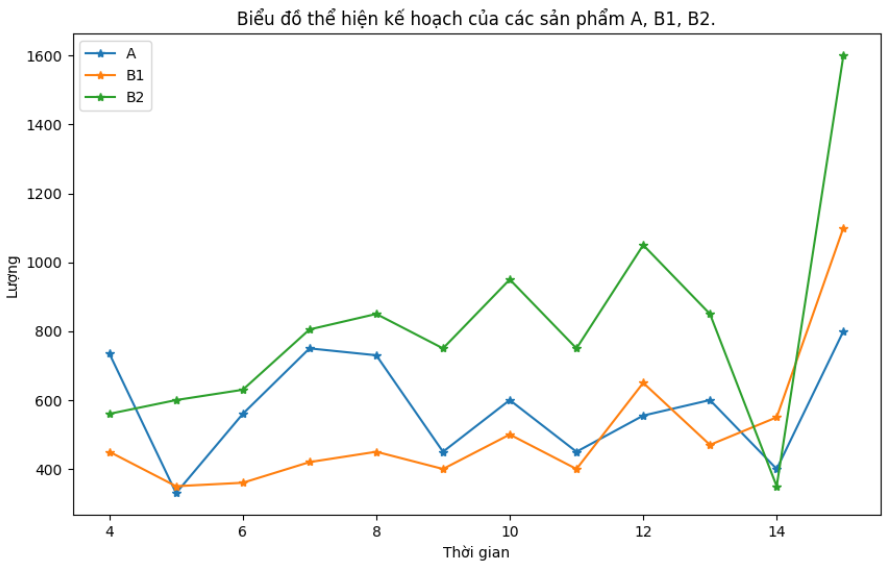
\includegraphics[width = 0.8\textwidth]{figure/AB1B2.png}
    \caption{Biểu đồ thể hiện số lượng của sản phẩm A, B1, B2 theo quý.}
    \label{fig:AB1B2}
\end{figure}

\begin{figure}[H]
    \centering
    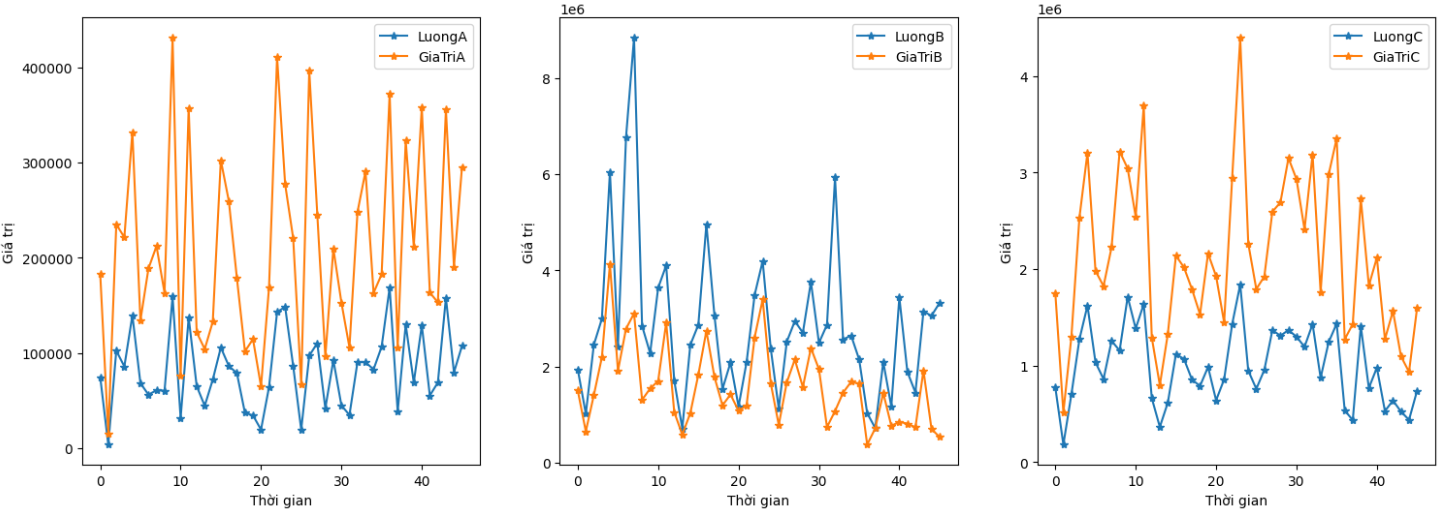
\includegraphics[width = \textwidth]{figure/ABCGiaTriLuong.PNG}
    \caption{Biểu đồ thể hiện sản phẩm A, B, C đối thủ theo tháng.}
    \label{fig:ABCGiaTriLuong}
\end{figure}

\section{Xử lý dữ liệu}
Do kế hoạch bên công ty là theo quý, còn đối thủ là theo tháng. Do đó gộp 3 tháng làm 1 quý và bỏ đi phần kế hoạch năm 2020 và tháng 10/2023 của đối thủ, quý 4 năm 2023 của công ty. Bỏ đi kế hoạch của sản phẩm C, và chỉ lấy phần lượng của mỗi sản phẩm A, B. Còn lại thu được 11 quý từ quý 1/2021 đến quý 3/2023. 

\begin{figure}[H]
    \centering
    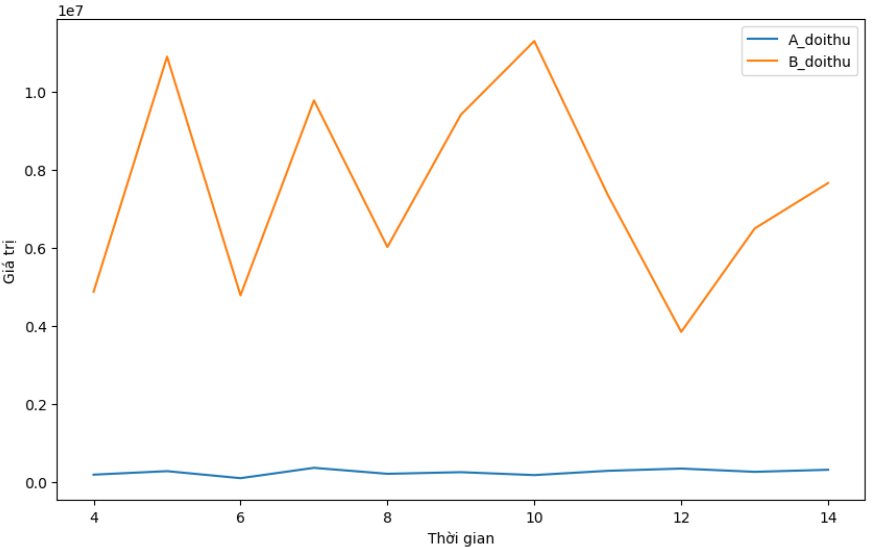
\includegraphics[width = \textwidth]{figure/ABLuong.PNG}
    \caption{Biểu đồ thể hiện sản phẩm A, B của đối thủ theo quý.}
    \label{fig:ABLuong}
\end{figure}

\section{Xây dựng mô hình}
Nhóm chia dữ liệu thành 2 tập train và test với train gốm 7 quý đầu, test gồm 4 quý sau. Và xây dựng, thử nghiệm các mô hình sau:
\begin{itemize}
        \item Sử dụng với 2 trường A, A đối thủ: VAR - OLS, VAR - Durbin-Levinson.
    \item Sử dụng với 3 trường B1, B2, B đối thủ: VAR - OLS, VAR - Durbin-Levinson.
    \item Sử dụng 5 trường A, B1, B2, A đối thủ, B đối thủ: VAR - OLS, VAR - Durbin-Levinson, Holt-Winters tối ưu theo Log-Likelihood, Holt-Winters tối ưu theo MSE.
\end{itemize}

\section{Kết quả thực nghiệm}
Qua quá trình thử nghiệm, nhóm sử dụng độ đo MAE thu được kết quả đánh giá sau:

% \begin{table}[H]
%     \centering
%     \resizebox{\textwidth}{!}
%         { 
%     \begin{tabular}{|l|l|l|l|l|l|l|l|l|l|l|}
%     \hline
%         Mô hình & A và A đối thủ & ~ & B1, B2 và B đối thủ & ~ & ~ & A, B1, B2, A đối thủ và B đối thủ & ~ & ~ & ~ & ~ \\ \hline
%         ~ & A & A đối thủ & B1 & B1  & B đối thủ & A & B1 & B2 & A đối thủ & B đối thủ \\ \hline
%         VAR & 63.608 & 99694.263 & 97.616 & 328.073 & 6814639.757 & 163.212 & 97.505 & 327.786 & 41173.739 & 6811127.587 \\ \hline
%         Durbin-Levinson & 111.328 & 74709.311 & 114.633 & 219.033 & 1928826.146 & 103.498 & 102.971 & 156.071 & 60742.338 & 2158559.805 \\ \hline
%         Holt-Winter tối ưu theo Log-likelihood & ~ & ~ & ~ & ~ & ~ & 245.501 & 57.501 & 339.251 & 97291.501 & 4844239.125 \\ \hline
%         Holt-Winter tối ưu theo MSE & ~ & ~ & ~ & ~ & ~ & 316.328 & 98.033 & 354.922 & 82337.041 & 9509946.258 \\ \hline
%     \end{tabular}
%     }
% \end{table}

\begin{table}[H]
    \centering
    \resizebox{\textwidth}{!}{ 
        \begin{tabular}{|c|c|c|c|c|c|c|c|c|c|c|}
        \hline
            \multirow{2}{*}{Mô hình} & \multicolumn{2}{c|}{A và A đối thủ} & \multicolumn{3}{c|}{B1, B2 và B đối thủ} & \multicolumn{5}{c|}{A, B1, B2, A đối thủ và B đối thủ} \\ \cline{2-11}
            & A & A đối thủ & B1 & B2  & B đối thủ & A & B1 & B2 & A đối thủ & B đối thủ \\ \hline
            VAR - OLS & \textbf{63.608} & 99694.263 & \textbf{97.616} & 328.073 & 6814639.757 & 163.212 & 97.505 & 327.786 & \textbf{41173.739} & 6811127.587 \\ \hline
            VAR - Durbin-Levinson & 111.328 & \textbf{74709.311} & 114.633 & \textbf{219.033} & \textbf{1928826.146} & \textbf{103.498} & 102.971 & \textbf{156.071} & 60742.338 & \textbf{2158559.805} \\ \hline
            Holt-Winter tối ưu theo Log-likelihood & & & & & & 245.501 & \textbf{57.501} & 339.251 & 97291.501 & 4844239.125 \\ \hline
            Holt-Winter tối ưu theo MSE & & & & & & 316.328 & 98.033 & 354.922 & 82337.041 & 9509946.258 \\ \hline
        \end{tabular}
    }
\end{table}

Kết quả dự báo $4$ quý tiếp theo trong năm $2024$ bằng mô hình Durbin-Levinson được biểu diễn trong bảng \ref{DB4nam2024}
\begin{table}[H]
    \centering
    \caption{Kết quả dự báo 4 quý năm 2024 bằng mô hình VAR - Durbin-Levinson.}
    \label{DB4nam2024}
    \resizebox{\textwidth}{!}{ 
        \begin{tabular}{|c|c|c|c|c|c|c|c|c|c|c|}
        \hline
            \multirow{2}{*}{Quý} & \multicolumn{2}{c|}{A và A đối thủ} & \multicolumn{3}{c|}{B1, B2 và B đối thủ} & \multicolumn{5}{c|}{A, B1, B2, A đối thủ và B đối thủ} \\ \cline{2-11}
            & A & A đối thủ & B1 & B2  & B đối thủ & A & B1 & B2 & A đối thủ & B đối thủ \\ \hline
            1 & 534.637 & 260718.824 & 456.899 & 757.619 & 8020657.233 & 529.176 & 458.487 & 760.954 & 271257.466  & 7956737.484 \\ \hline
            2 & 572.094 & 236579.687 & 453.417 & 734.091 & 7291676.408 & 580.709 & 460.710 & 747.793 & 229189.165 & 7025864.153 \\ \hline
            3 & 554.189 & 248210.334 & 454.772 & 741.086 & 7565733.786 & 540.675 & 451.292 & 741.719 & 258889.882 & 7832721.811  \\ \hline
            4 & 562.794 & 242614.486 & 454.436 & 740.095 & 7451979.116 & 575.599 & 457.979 & 741.555 & 232923.170 & 7195879.347 \\ \hline
        \end{tabular}
    }
\end{table} 
\begin{figure}[H]
    \centering
    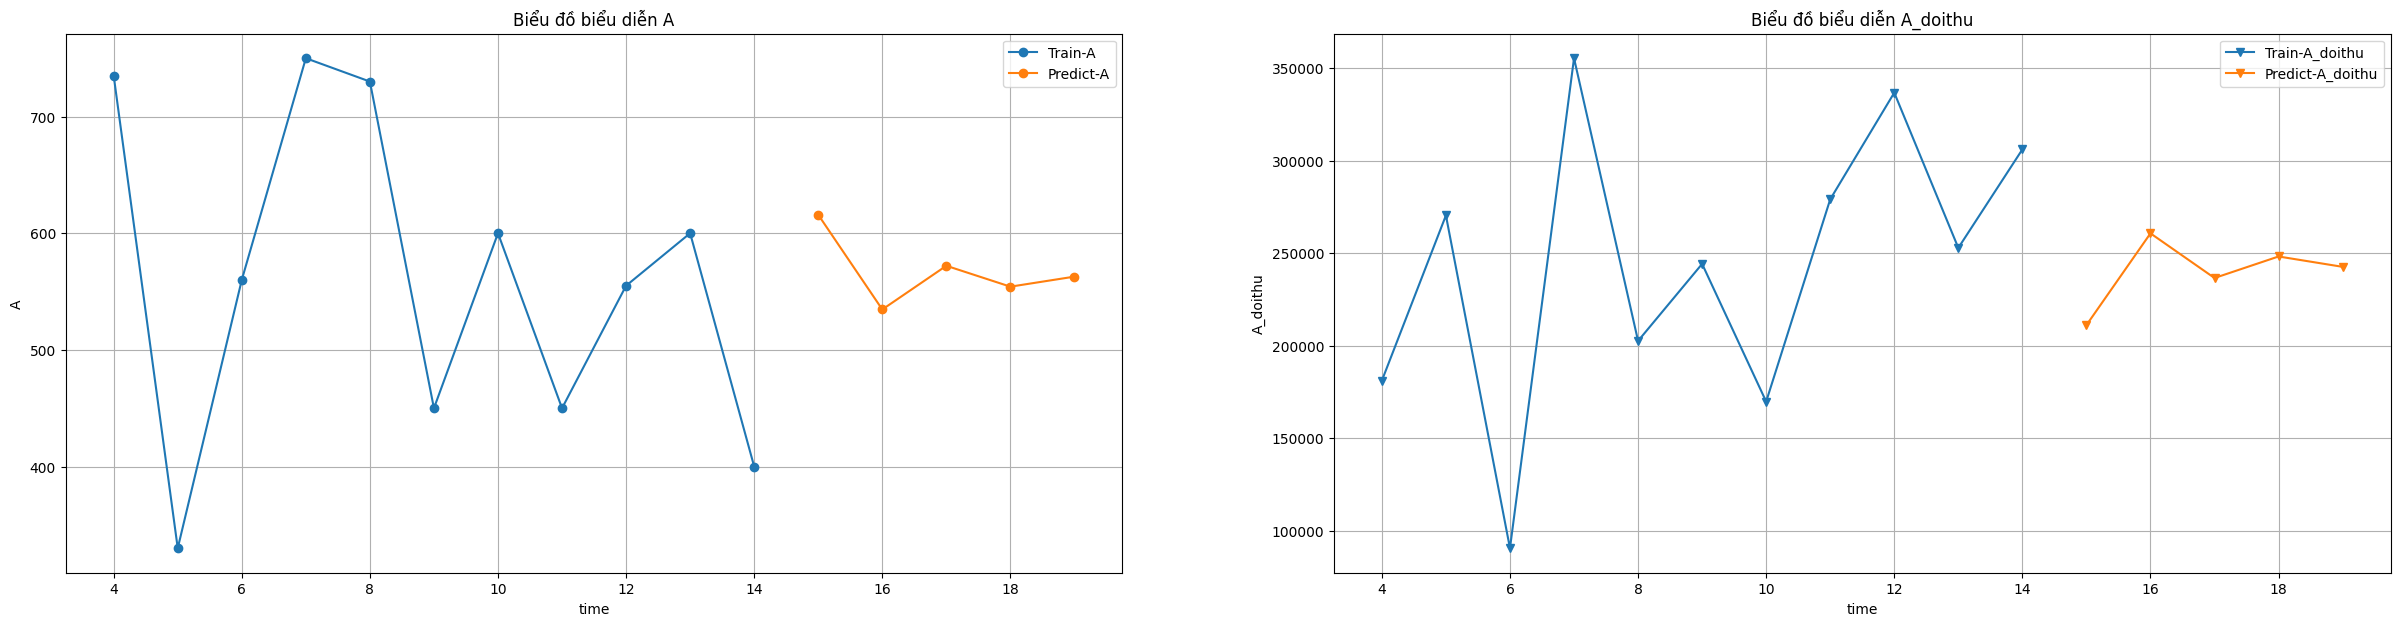
\includegraphics[width = \textwidth]{figure/preDB2.png}
     \caption{Kết quả dự đoán các quý tiếp theo của mô hình VAR - Durbin-Levinson trên 2 trường A và A đối thủ.}
\end{figure}
\begin{figure}[H]
    \centering
    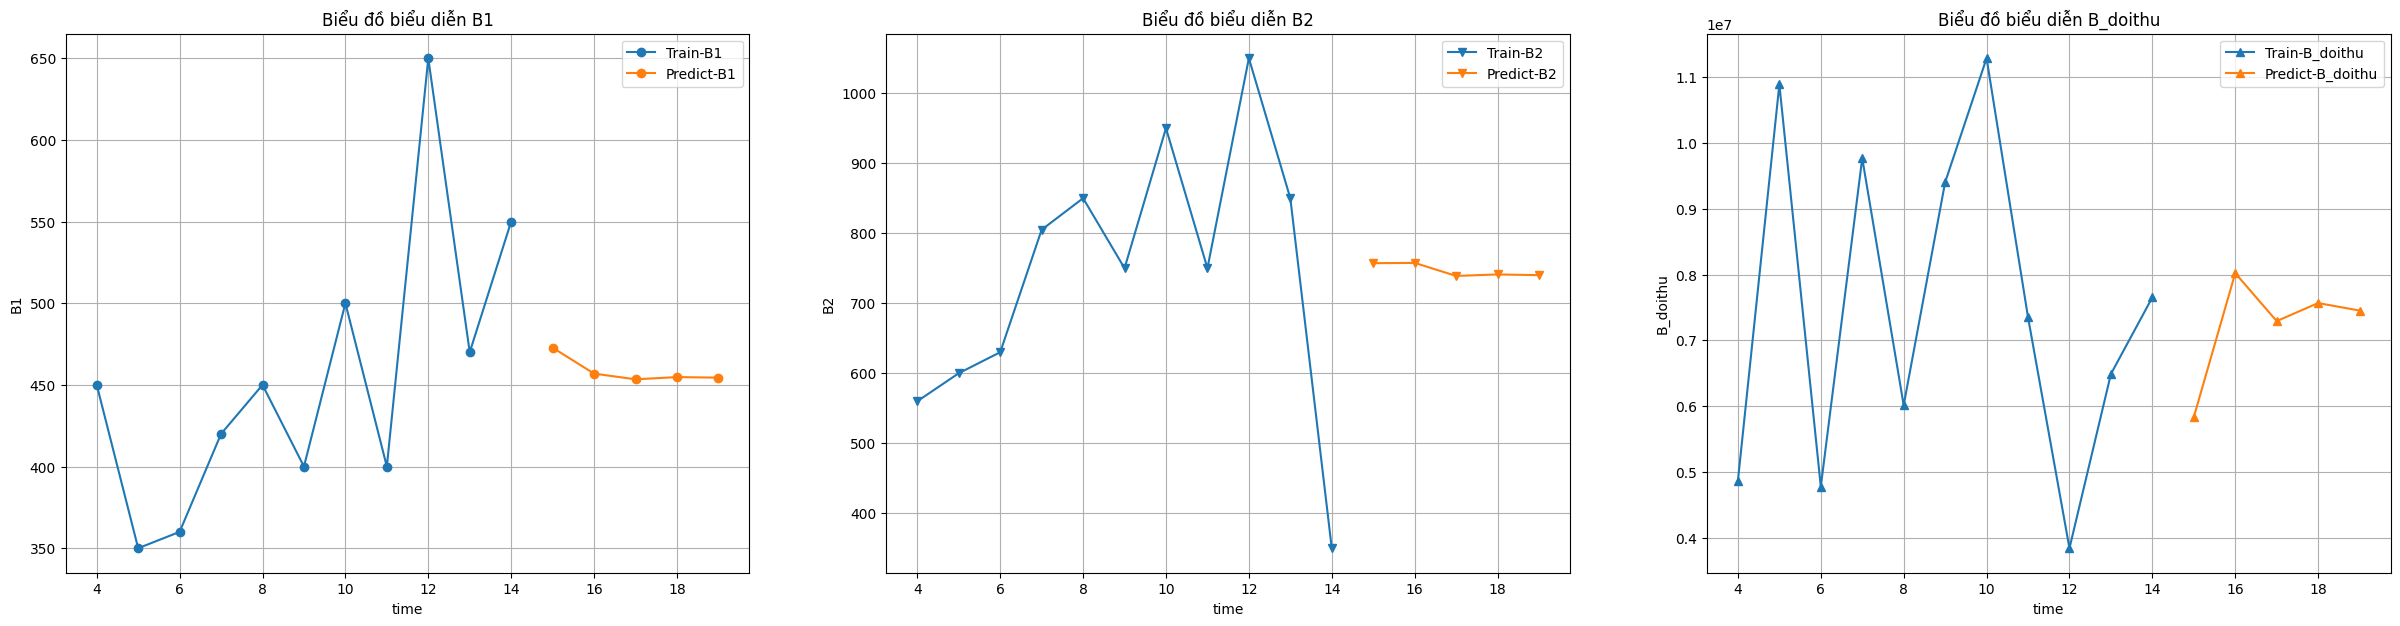
\includegraphics[width = \textwidth]{figure/preDB3.png}
     \caption{Kết quả dự đoán các quý tiếp theo của mô hình VAR - Durbin-Levinson trên 3 trường B1, B2 và B đối thủ.}
\end{figure}

\begin{figure}[H]
    \centering
    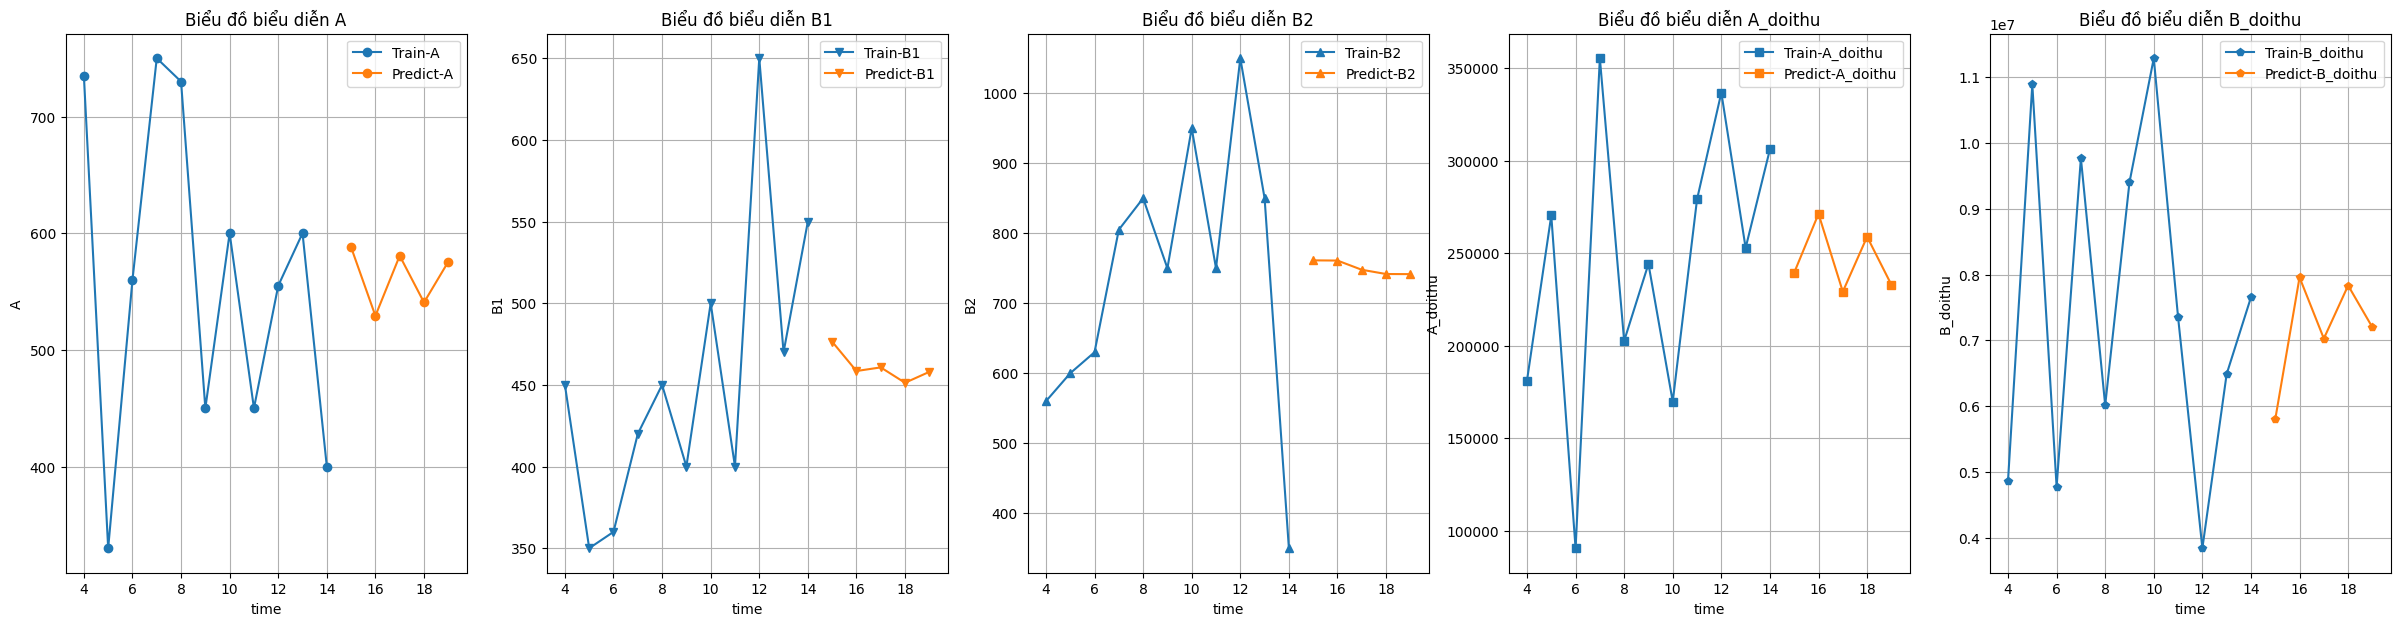
\includegraphics[width = \textwidth]{figure/preDB5.png}
     \caption{Kết quả dự đoán các quý tiếp theo của mô hình VAR - Durbin-Levinson trên cả 5 trường.}
\end{figure}
Kết quả dự báo $4$ quý liên tiếp của năm $2024$ theo phương pháp Holt-Winters có trong bảng \ref{HL4nam2024} và \ref{HM4nam2024}. 
\begin{table}[H]
    \centering
    \caption{Kết quả dự báo 4 quý năm 2024 bằng mô hình Holt-Winters tối ưu theo hàm Log-Likelihood.}
    \label{HL4nam2024}
    \resizebox{\textwidth}{!}{ 
        \begin{tabular}{|c|c|c|c|c|c|}
        \hline
         Quý & A & B1 & B2 & A đối thủ & B đối thủ  \\ \hline
         1 & 611.179 & 667.743 & 945.461 & 337227.027 & 3748242.589 \\ \hline
         2 & 398.308 & 557.512 & 858.160 & 352909.032 & 7769289.737 \\ \hline
         3 & 458.769 & 620.615 & 767.525 & 285877.371 & 6748481.551 \\ \hline
         4 & 522.308 & 598.846 & 934.326 & 438602.865 & 7113320.903 \\ \hline
        \end{tabular}
    }
\end{table} 

\begin{figure}[H]
    \centering
    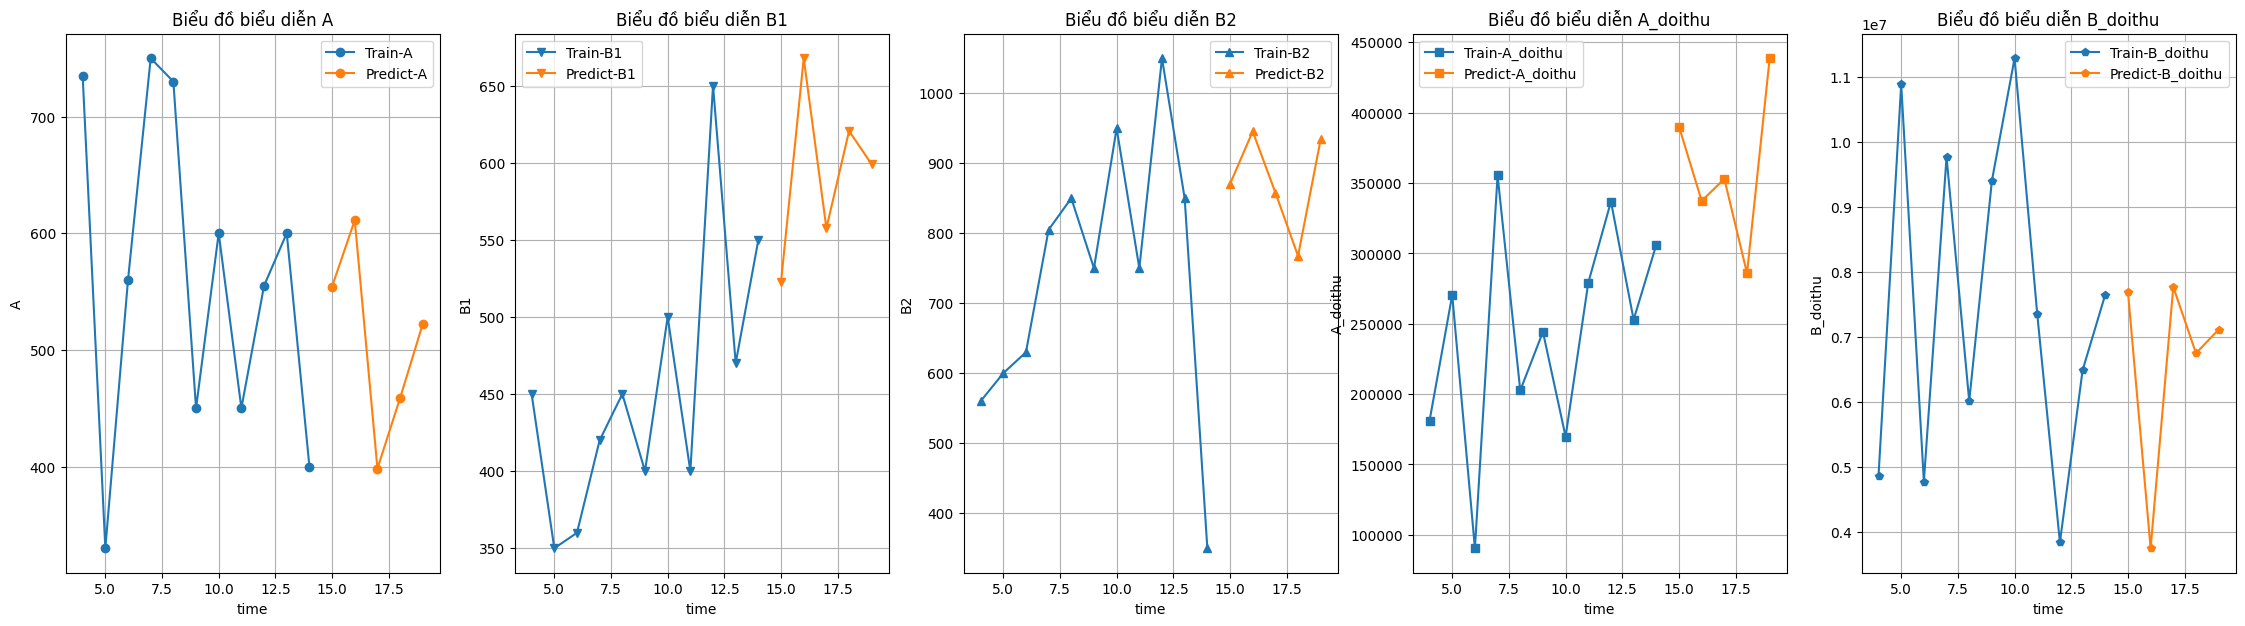
\includegraphics[width = \textwidth]{figure/HW-likelihood.png}
     \caption{Kết quả dự đoán 4 quý năm 2024 bằng mô hình Holt-Winters tối ưu theo hàm Likelihood.}
\end{figure}

\begin{table}[H]
    \centering
    \caption{Kết quả dự báo 4 quý năm 2024 bằng mô hình Holt-Winters tối ưu theo hàm MSE.}
    \label{HM4nam2024}
    \resizebox{\textwidth}{!}{ 
        \begin{tabular}{|c|c|c|c|c|c|}
        \hline
         Quý & A & B1 & B2 & A đối thủ & B đối thủ  \\ \hline
         1 & 783.931 & 782.078 & 1181.535 & 408328.905 & 6563700.954 \\ \hline
         2 & 549.187 & 671.608 & 1103.708 & 431537.413 & 10697519.506 \\ \hline
         3 & 623.912 & 726.248 & 1034.390 & 354718.765 & 9344292.680 \\ \hline
         4 & 741.065 & 751.774 & 1263.108 & 541828.309 & 10713969.767 \\ \hline
        \end{tabular}
    }   
\end{table} 

\begin{figure}[H]
    \centering
    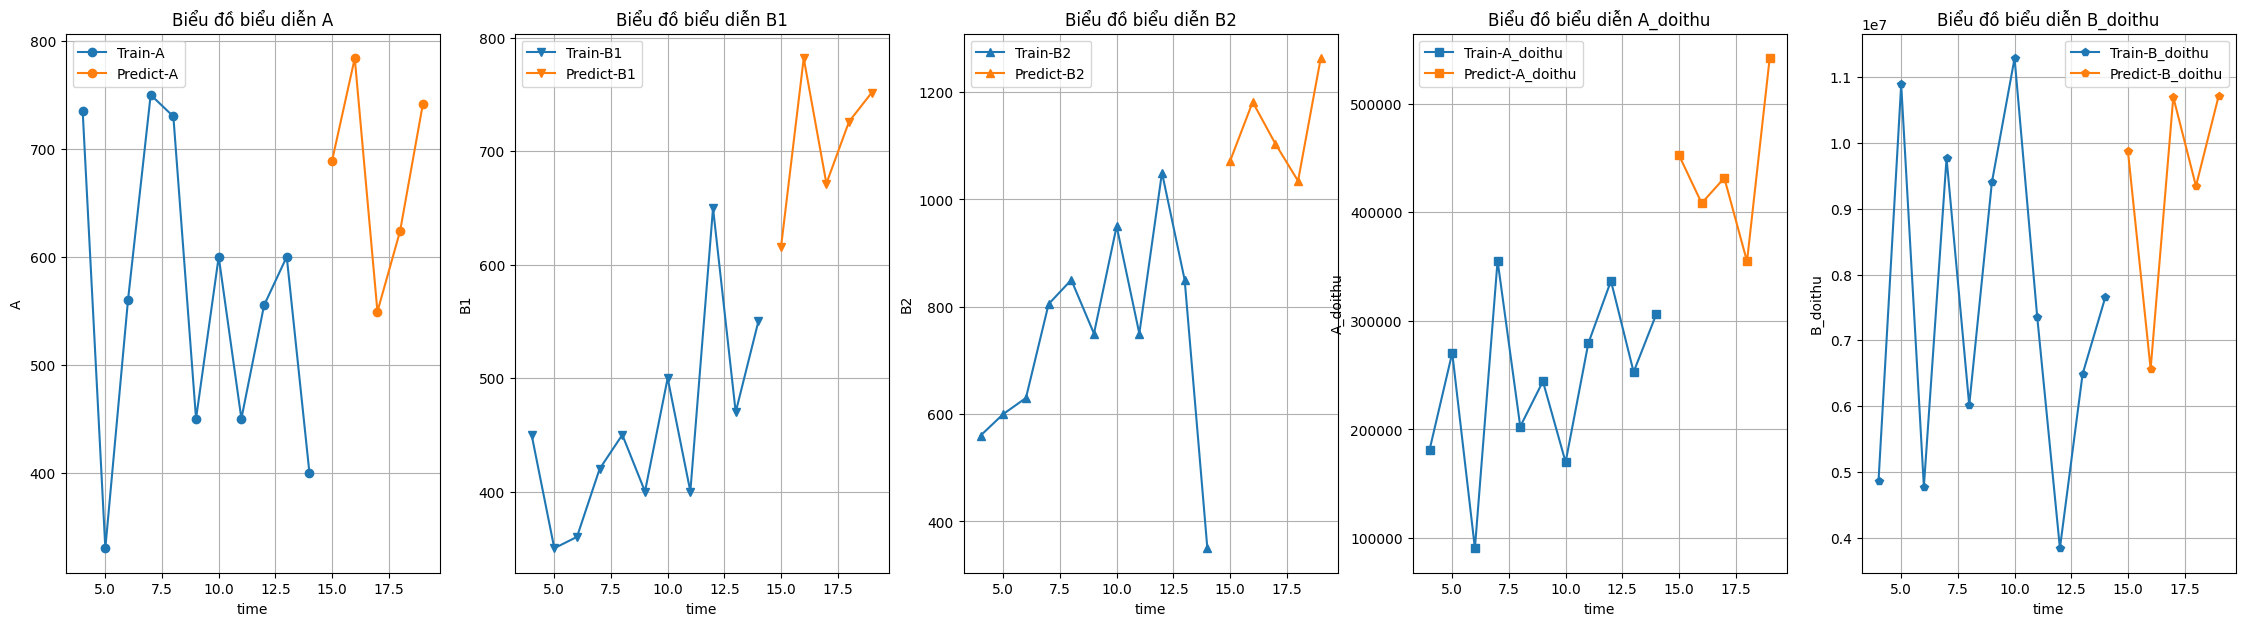
\includegraphics[width = \textwidth]{figure/HW-mse.png}
    \caption{Kết quả dự báo 4 quý năm 2024 bằng mô hình Holt-Winters tối ưu theo hàm MSE.}
\end{figure}

\begin{table}[H]
    \centering
    \caption{Kết quả dự báo 4 quý năm 2024 bằng mô hình VAR - OLS.}
    \label{DB4nam2024}
    \resizebox{\textwidth}{!}{ 
        \begin{tabular}{|c|c|c|c|c|c|c|c|c|c|c|}
        \hline
            \multirow{2}{*}{Quý} & \multicolumn{2}{c|}{A và A đối thủ} & \multicolumn{3}{c|}{B1, B2 và B đối thủ} & \multicolumn{5}{c|}{A, B1, B2, A đối thủ và B đối thủ} \\ \cline{2-11}
            & A & A đối thủ & B1 & B2  & B đối thủ & A & B1 & B2 & A đối thủ & B đối thủ \\ \hline
            1 & 501.369 & 430125.909 & 480.701 & 835.505 & 4878039.48 & 477.249 & 480.841 & 835.488 & 272521.765 & 4880684.39 \\ \hline
            2 & 704.477 & 384310.265 & 480.906 & 671.971 & 4877756.56& 438.670 & 481.041 & 672.221 & 259961.421 & 4880244.12 \\ \hline
            3 & 611.613 & 386588.924 & 431.586  & 443.055 & 4813185.67 & 345.854 & 431.746 & 443.405 & 233389.177 & 4817447.48 \\ \hline
            4 & 638.573 & 429640.797 & 352.013  & 451.676 & 4893416.66 & 335.253 & 352.348 & 451.911 & 203718.448 & 4897584.47 \\ \hline
        \end{tabular}
     }
\end{table} 

\begin{figure}[H]
    \centering
    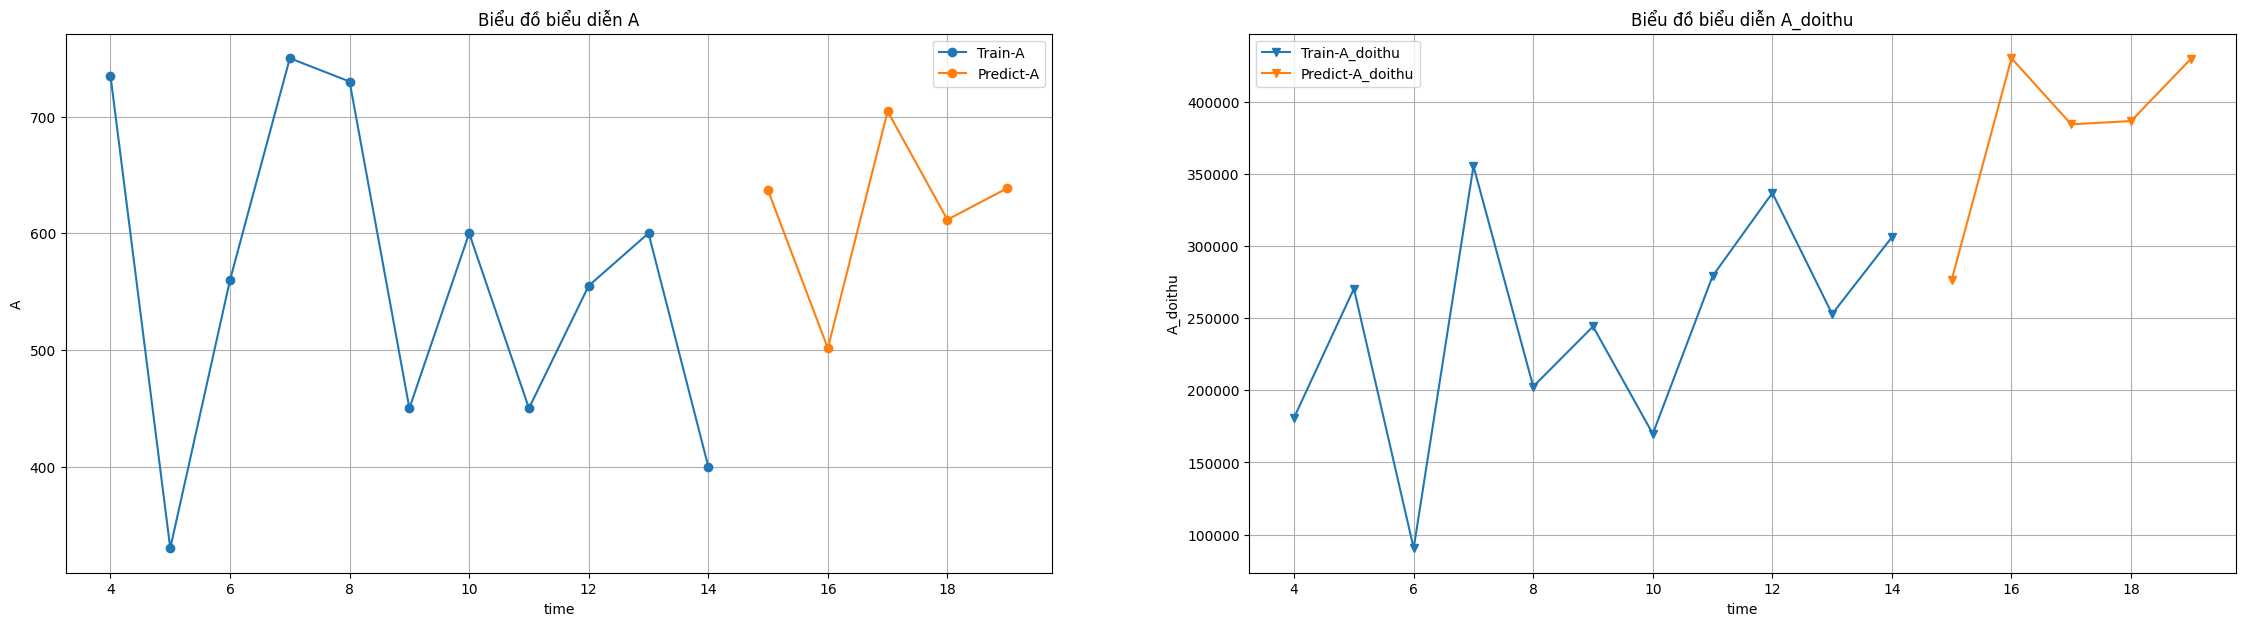
\includegraphics[width = \textwidth]{figure/VAR2.png}
    \caption{Dự đoán 4 quý năm 2024 của mô hình VAR - OLS trên 2 trường A và A đối thủ.}
    \label{fig:var2}
\end{figure}

\begin{figure}[H]
    \centering
    \includegraphics[width = \textwidth]{figure/VAR3.png}
    \caption{Dự đoán 4 quý năm 2024 của mô hình VAR - OLS trên 3 trường B1, B2 và B đối thủ.}
    \label{fig:var2}
\end{figure}

\begin{figure}[H]
    \centering
    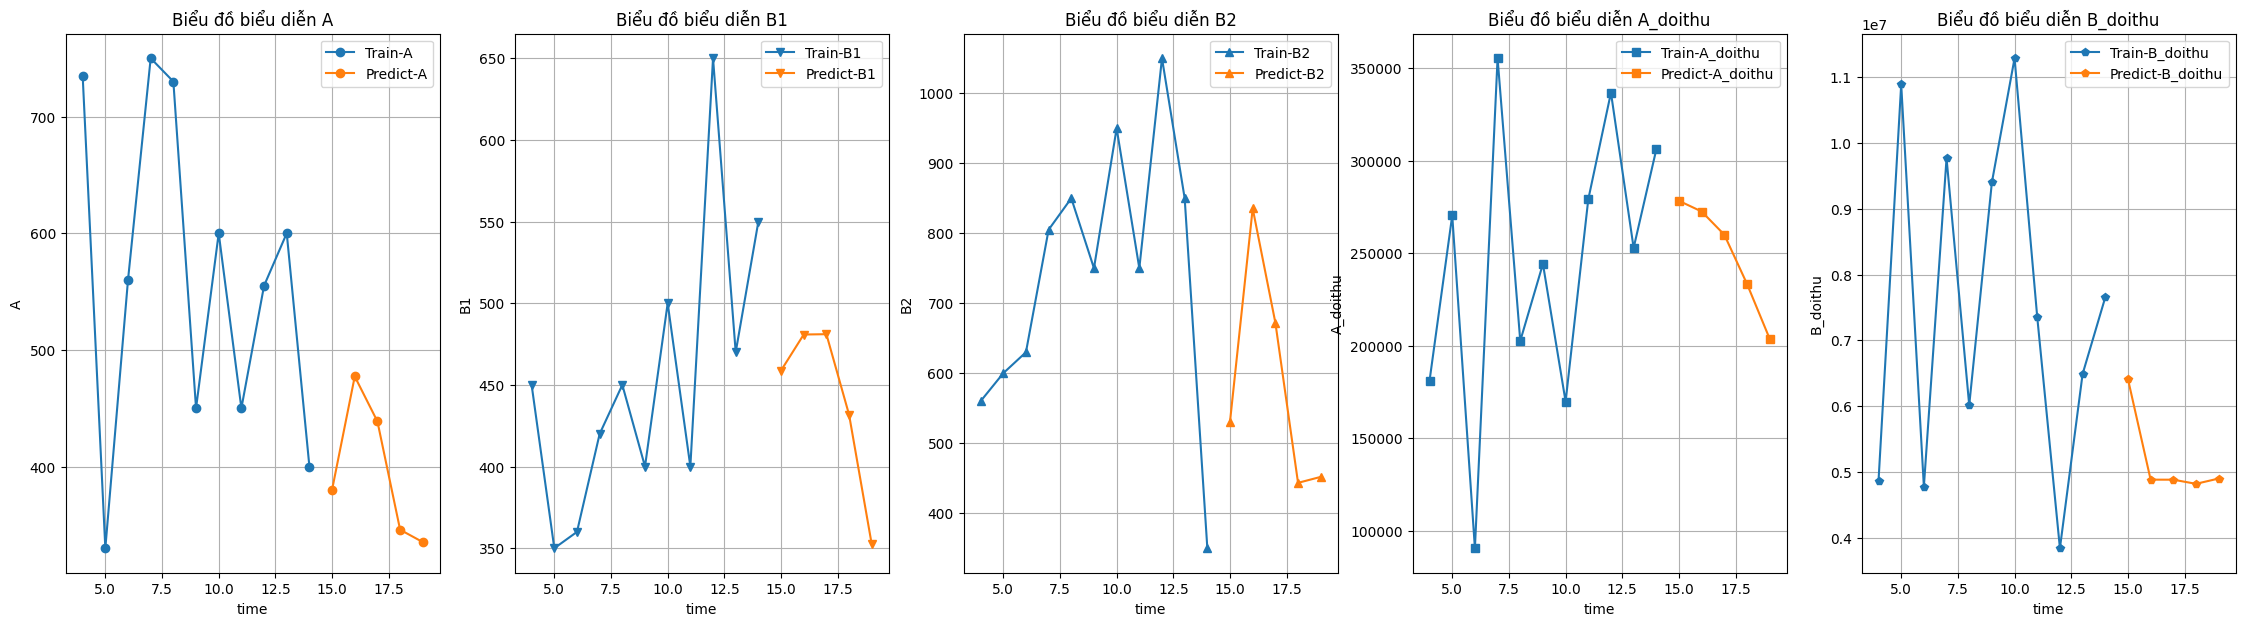
\includegraphics[width = \textwidth]{figure/dudoanVAR.png}
    \caption{Dự đoán 4 quý năm 2024 tiếp theo của mô hình VAR - OLS trên cả 5 trường.}
    \label{fig:var5}
\end{figure}
	\chapter{KẾT LUẬN}
Trong phạm vi nội dung của đồ án, một số nội dung mà nhóm chúng em đã đạt được:
\begin{itemize}
    \item Thành công trong việc giới thiệu 2 mô hình dự đoán chuỗi thời gian VAR và Holt-Winters. 
    \item Ứng dụng được vào bài toán dự báo nhu cầu sản phẩm.
    \item So sánh được hiệu quả của mô hình VAR và Holt-Winters trong bài toán dự báo nhu cầu sản phẩm.
\end{itemize}
Với những kết quả đạt được, đồ án có nhiều tiềm năng ứng dụng trong nhiều bài toán khác nhau về chuỗi thời gian. Một số hướng phát triển tiếp theo của đồ án:
\begin{itemize}
    \item Cải thiện độ chính xác của mô hình và ứng dụng vào nhiều lĩnh vực khác nhau, ví dụ: dự báo tỉ lệ người nhiễm covid, dự đoán doanh số bán hàng, v.v...
    \item Ứng dụng các mô hình học sâu để giải quyết bài toán.
\end{itemize}


	
\begin{thebibliography}{99}\rm
\addcontentsline{toc}{chapter}{\bf Tài liệu tham khảo}
\bibitem{Ber2007} Bermúdez. J. D., Segura, J. V., \& Vercher, E. , Holt–Winters forecasting: an alternative formulation applied to UK air passenger data, \textit{Journal of Applied Statistics}, 34(9), 1075-1090, 2007.
\bibitem{Jones1978} Jones. R. H.,  Multivariate autoregression estimation using residuals. \textit{In Applied Time Series Analysis I} (pp. 139-162). Academic Press, 1978.

\bibitem{HELMUT2005} \text{Helmut L\"utkepohl}, \textit{New Introduction to Multiple Time Series Analysis}, Springer Berlin, Heidelberg, 2005.

\end{thebibliography}


	
\end{document}
